\begin{document}

\section{Percentage Price Oscillator}

Im Nachfolgenden wurde die Umsetzung des ’Percentage Price Oscillator’-Indikators (kurz: PPO) in ein vorhandenes Warehouse-Komplexes untersucht. Dieses Warehouse hatte zum Ziel auf Basis von mehreren Indikatoren (Entscheidungsfaktoren) in einem nicht genauer bestimmten Zeitraum automatisierte Aktien-Transaktionen mit höchstmöglichen Nettoresultat durchzuführen.

\subsection{Definition}
Der PPO gehört zu der Indikator Kategorie der Momentum-Oszil\-latoren, die auf der Annahme basieren, dass bei nachlassendem Momentum das Handelsvolumen nachlässt und vice versa. Daraus lassen sich diverse Handlungsentscheidungen sowie Handlungsimpulse ableiten, welche dieser Indikator mit Hilfe von hauptsächlich zwei gleitenden Durchschnitten unterschiedlicher Länge versucht zu bestimmen.

Der PPO ist hierbei dem 'Moving Average Convergence/Divergence' (kurz: MACD) sehr ähnlich, unterscheidet sich aber im Wertebereich, welche bei dem PPO prozentual ist. Diese Tatsache ermöglicht eine wesentliche einfachere Vergleichbarkeit von Kursen über einen längeren Zeitraum hinweg.

\subsection{Umsetzung}
Die Umsetzung eines solchen Indikator lässt sich in 4 wesentliche Schritten unterteilen. Zuallererst müssen Daten in das Subsystem zugeführt werden, welches für das Bestimmen des Indikators zuständig ist. Anschließend können auf Basis der Inputdaten und unterschiedlicher, parametrisierbaren Faktoren der PPO-Indikator berechnet werden. Ausgehend von dieser Berechnung können Handlungsanweisungen als Analyseresultat aggregiert werden, welche in einem letzten Schritt dem Warehousesystem übergeben werden. Für die Entwicklung des Systems und zu Präsentationszwecken empfiehlt sich zudem ein weiterer Schritt: die graphische Aufbereitung der Daten. Im Nachfolgenden werden dieser Schritte näher betrachtet.

\subsubsection{Datenzufuhr und Datengrundlagen} 
\label{subsec_datenbase_ppo}
Je nach Warehouse-Design und Ausgangslage müssen für die Zufuhr einer Datenbasis bereits von Datenquellen Selektierungs- oder Aggregationsoperationen Durchgeführt werden. Hierzu empfiehlt es sich aber einen dedizierten Layer zur Aufbereitung und Falsifizierung der Daten (vgl. Interpolation) zu verwenden. 
Da bei diesen Projekt mehrere Aktienkurse untersucht werden sollen, ist es zwingend erforderlich, in dem dafür zuständigen Dataframe Spalten für die Identifikation eines Kurses (Aktienname) und Kursdaten (Closing-, Opening-,  High-, Low- sowie Volumenwerte) zu haben. Zusätzlich bedarf es einer Spalte mit einem passenden Datentypen, der den jeweiligen Zeitpunkt repräsentiert.

\subsubsection{Berechnung}
\label{subsec_berrechnung_ppo}
Wie erwähnt benutzt der PPO zwei gleitende Durchschnitte, diese dienen als sogenannte Nachlaufindikatoren und umfassen i.d.R. 26 und 12 aufeinander folgende Werten eines Kurses. Als Basis der Werte bietet sich der Closing-Wert bei einer tagesbasierten Implementation an. Als gleitender Durchschnitt empfiehlt sich der häufig verwendete 'Exponential Moving Average' (kurz: EMA), welcher im Vergleich zum 'Simple Moving Average' (kurz: SMA) den letzten Wert mehr Bedeutung beimisst. Dadurch schlägt dieser Indikator etwas schneller auf Kursänderungen aus. Alternativ dazu könnten auch der 'Weighted Moving Average' (kurz: WMA) oder der 'Displaced Moving Average' (kurz: DMA) und andere angewandt werden. Für die weiteren Abschnitte wird die Implementation mit dem aus EMA berechneten gleitenden Durchschnitt angewandt auf von 26 bzw. 12 aufeinander folgenden Werten beschrieben. 

Der PPO Indikator besteht aus drei zu bestimmenden Werten: dem PPO-Wert, dem Signal-Wert und einer daraus resultierenden Vergleichs-Wert. Der PPO-Wert wird als Differenz der beiden EMA-Werte im Verhältnis zu den größeren Werte umfassenden Durchschnitt, als prozentualer Wert bestimmt. Aus dem EMA mit 26 und 12 historischen Werten lässt sich also der PPO-Wert bestimmen und so anschließend darauf aufbauend, mit ebenfalls dem gleitenden Durchschnitt - hierbei i.d.R. 9 vergangen Werten des PPO-Werts - der sog. Signalwert. Abschließend lässt sich aus der Differenz dieser beiden Werten der Vergleichs-Wert bestimmen; dieser bildet ein Histogramm des PPO- und Signal-Wertes. (s. Abb. ~\ref{fig:formular_ppo})

\begin{figure}[!ht]
\begin{gather*} 
PPO = ( EMA_{12}(close) - EMA_{26}(close) ) / EMA_{26}(close) * 100 \\ 
SIGNAL =  EMA_9( PPO )\\
VERGLEICHSWERT = PPO - SIGNAL
\end{gather*}
\caption{Berechnungsformeln für den Percentage Price Oscillator}
\label{fig:formular_ppo}
\end{figure}

\subsubsection{Analyse}
\label{subsec_analysis_ppo}
In einem nächsten Schritt lassen sich die aus der PPO-Berechnung entstehenden Daten analysieren. Dieser Schritt lässt sich wiederum in zwei Teilschritte untergliedern: dem bestimmen der Entscheidungsfaktoren und dem zusammenführen dieser zu einem einzigen Wert.

\subsubsubsection{Determinieren der Entscheidungsfaktoren}
\label{subsubsec_analysis_calc_ppo}
Für die Analyse lassen sich 4 Faktoren mit unterschiedlicher Gewichtung bestimmen. Basierend auf einem spezifischen PPO-Wert im Vergleich zu seinen vorherigen lässt sich ein Trend bestimmen (s. Abb. ~\ref{fig:trendbestimmung_ppo}).

\begin{figure}[!ht]
\begin{lstlisting}[language=Python,numbers=auto]
# ...
if last > 0 and next_to_last > 0:
 output = "Aufwärtstrend"
elif last < 0 and next_to_last > 0:
 output = "neuer Abwärtstrend"
elif last < 0 and next_to_last < 0:
 output = "Abwärtstrend"
elif last > 0 and next_to_last < 0:
 output = "neuer Aufwärtstrend"
# ...
\end{lstlisting}
\caption{Trendbestimmung für den Percentage Price Oscillator}
\label{fig:trendbestimmung_ppo}
\end{figure}

Des Weiteren lässt sich anhand der Nullpunkte im Verlauf des PPO-Wertes das sog. Weaksignal ermitteln - anhand der Nullpunkte im Histogramms leitet sich das sog. Strongsignal ab. Hierbei gilt: Schneidet der aus dem Verlauf resultierende Graph den Nullpunkt aus einem negativen Wertebereich heraus, handelt es sich um ein Kaufsignal - kommt er hingegen aus einem Positiven, handelt es sich um ein Verkaufssignal (s. Abb. ~\ref{fig:signalbestimmung_ppo}).

Anschließend lässt sich noch die Divergence als Analysefaktor nutzen: Hierbei wird die Steigung des aus dem Verlauf resultierende Graphen der PPO-Werte mit dem ursprünglich zur PPO-Berechnung genutzten Wert verwendet (hier der Closing-Wert). Steigt der Closing-Wert schneller als der PPO-Wert, handelt es sich um einen abflachenden Trend - steigt der PPO-Graph hingegen schneller handelt es sich um wachsenden Trend. 

\begin{figure}[!ht]
\begin{lstlisting}[language=Python,numbers=auto]
# ...
if last <= 0 and next_to_last > 0:
 output = "Verkauf-Signal"
elif last >= 0 and next_to_last < 0:
 output = "Kauf-Signal"
# ...
\end{lstlisting}
\caption{Signalbestimmung für den Percentage Price Oscillator}
\label{fig:signalbestimmung_ppo}
\end{figure}

\subsubsubsection{Kombinieren der Entscheidungsfaktoren}
\label{subsubsec_analysis_comb_ppo}
Für das kombinierte Analyseergebnis ist der Datentyp zur Übergabe im Warehouse maßgeblich; Hieraus resultiert zwangsläufig, dass dieser Schritt für jedes Projekt in höchsten Maße differenziert zu betrachten ist. Als Datentyp für einen Tradingbot, wie es in diesem Projekt durch das Warehousekomplex vorgeben ist, empfiehlt sich eine Codierung der Handlungsmuster des Bots und eine direkt dazugehörige Codierung des Grades der Handlungsempfehlung.

Allerdings lässt sich aus den zuvor determinierten Entscheidungsfaktoren ein Gewichtungsfaktor ableiten: Der wichtigste Faktor der sog. 'Trend', gefolgt von dem Strong- und Weak-Signal (s. Abb. ~\ref{fig:faktorenhierrachie_ppo}). Eine genaue Gewichtung der genannten Faktoren kann durch eine fortwährende Analyse der Ergebnisse innerhalb des gesamten Projekt bestimmt werden.

\begin{figure}[!ht]
\begin{eqnarray}
G_{Trend} \geq  G_{Strongsignal} \approx G_{Weaksignal} \geq G_{Divergence}\nonumber
\end{eqnarray}
\caption{Gewichtung der Entscheidungsfaktoren für den Percentage Price Oscillator}
\label{fig:faktorenhierrachie_ppo}
\end{figure}

\subsubsection{Graphische Aufbereitung}
Eine graphische Aufbereitung der berechneten Daten in einem Produktions-Warehouse ist aufgrund der Datengröße i.d.R. zu vermeiden. Aufgrund der Programmierkomplexität der graphischen Darstellung empfiehlt es sich in Abhängigkeit von Programmierumgebung und -sprache eine für Aktienkurse taugliche (opensource) Bibliothek zu nutzen. 

Um ein Kerzendiagramm (s. Abb. ~\ref{graph_btcusd_ppo_2}) für den allgemeinen Kursverlauf darzustellen, bzw. in ein Liniendiagramm (s. Abb. ~\ref{graph_btcusd_ppo_1}) für die PPO- und Signal-Werte, sowie ein Säulendiagramm für die Vergleichs-Werte, müssen nach Datenimport (s. Abs. ~\ref{subsec_datenbase_ppo}), Berechnung (s. Abs. ~\ref{subsec_berrechnung_ppo}) und Analyse (s. Abs. ~\ref{subsec_analysis_ppo}) keine weiteren Daten aufbereitet oder berechnet werden, sofern keine Filteroperationen durchgeführt werden müssen.

\begin{figure}[!htb]
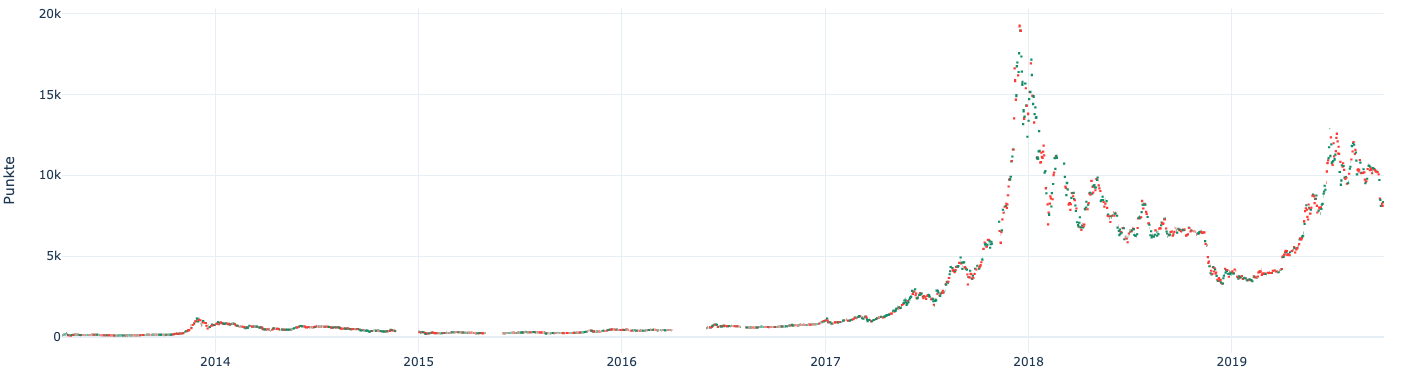
\includegraphics[width=.5\textwidth,keepaspectratio]{ppo/graph_btcusd_ppo_2}
\caption{Kerzendiagramm 'BTC-USD', (Veränderungen in Punkten)}
\label{graph_btcusd_ppo_2}
\end{figure}

\begin{figure}[!htb]
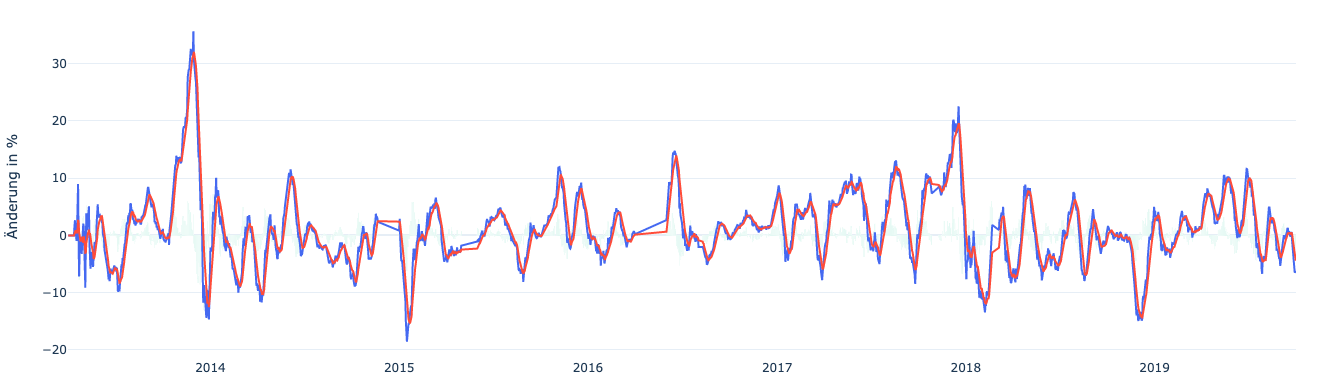
\includegraphics[width=.5\textwidth,keepaspectratio]{ppo/graph_btcusd_ppo_1}
\caption{Liniendiagramm 'BTC-USD', (Änderung in \%; blau: PPO, rot: Signal)}
\label{graph_btcusd_ppo_1}
\end{figure}

\subsubsection{Weitergabe der Daten}
Die Form der weiterzugebenden berechneten Daten erfolgt in Abhängigkeit des Warehousekomplexes. Für eine optimiertes, auf einem Cluster basierendes Warehouse und clusterbasierendes Subsystem, welches zuständig für die Weitergabe der Daten ist, empfiehlt es sich aufgrund der Datenmengen, diese als partitioniertstrukturierte Daten zu schreiben und anderen Subsystem zur Verfügung zustellen. Möchte man solche Daten jedoch menschlich-leicht-lesbar zur Verfügung stellen, so lassen diese sich leicht mit diversen Shell-Befehlen kombinieren.

Als konkreter Dateityp empfiehlt sich CSV oder Parquet. CSV-Dateien sind zeilenbasiert und damit leicht menschlichlesbar, skalieren aber bei großen Datenmengen (ab ca. 70.000 Zeilen) i.d.R. nicht gut, mit Folgen für das gesamte Laufzeitverhalten. Parquet-Dateien sind hingegen spaltenbasiert, daraus resultiert eine wesentlich geringere Latenz bei Leseoperationen, wie sie bei der Berechnung des PPO's zum Einsatz kommen. Da bei diesem Projekt der Forschungsnutzen und damit die Lesbarkeit im Vordergrund stand wurden die Daten im CSV-Format exportiert.

\subsection{Durchführung}
Für die Durchführung wurde PySpark verwendet, da diese überausreichend Funktionalität, Leistungsfähigkeit und Unterstützung verfügt. Als Entwicklungsumgebung wurde Google Colaboratory aufgrund der schnellen und einfachen Nutzbarkeit genutzt; als finale Laufzeitumgebung kamen Server von AWS (Amazon Web Services) zum Einsatz, da hier genügend Leistung verfügbar war, um den vorhanden Datensatz zeitnah bearbeiten zu können.

Die Berechnung des EMAs (s. Abs. ~\ref{subsec_berrechnung_ppo}) wurde als UDF (user-defined-function) implementiert. In Verbindung mit Window-Funk\-tionen (s. Abb. ~\ref{fig:formular_ppo}; über jeweils parametrisierbare Spaltenanzahl; hier: 26,12 bzw. 9) können anschließend alle benötigten Werte (s. Abb. ~\ref{fig:formular_ppo}) bestimmt werden.
Für die Analyse (s. Abs. ~\ref{subsec_analysis_ppo}) kamen Window-Funktionen zum Einsatz über mindestens 2 Spalten. Hierfür wurden desweiteren 3 UDF implementiert (die Berechnung des Strongsignals sowie des Weaksignals erfolgt mittels identischer Implementation, s. Abs. ~\ref{subsubsec_analysis_calc_ppo}). Für das anschließende Kombinieren dieser Analysefaktoren (s. Abs. ~\ref{subsubsec_analysis_comb_ppo}) wurde ein entsprechendes ausführliches SQL-Statemen, basierend auf dem CASE-Statement, definierten.
Um möglichst schnell (also u.a. resourcenschonender) alle CSV-Daten zu schreiben, wurde hierfür ein separates Python-Script erstellt. Dazu wurde zunächst die vorhanden Daten in einer große CSV-Datei kombiniert und dem Hadoop-Distributed-File-System (kurz: HDFS) zur Verfügung gestellt, um anschließend den nun nicht mehr benötigten Spark-Context zu beenden. 

Mit einem neuem Spark-Context wurde anschließend der etwa einstündige Schreibprozess gestartet (bei einem 5 Nodes großen Cluster für 2491 Tage bei bis max. 400 Kursdaten pro Tag). Abschließend wurden die tagebasierten berechneten Dateien (hier mit Headerschema) vom HDFS kopiert und mit Bash-Skript in eine leicht lesbare Form gebracht und dem Warehouse zur weiteren Verarbeitung zur Verfügung gestellt. 

\end{document}
